\input{aula}

\begin{document}

\title[PC1-01 Introdução]{
  {\large Programação de Computadores 1}\\[2mm]
  
\includegraphics[height=2cm]{images/scilab.png}\\
  {\normalsize Capítulo 1}\\
  Introdução ao Scilab
}
\subject{Programação de Computadores}
\author{José Romildo Malaquias}
\institute[UFOP]{
  Departamento de Computação\\
  Universidade Federal de Ouro Preto
}
\date{\semester}

\frame{\titlepage}

\frame{\tableofcontents}



\section{MATLAB e Scilab}

\begin{frame}[allowframebreaks]{MATLAB}
  \begin{itemize}
    \item \textbf{MATLAB} é uma \alert{linguagem} de alto nível e um
    \alert{ambiente interativo} para computação numérica, visualização e
    programação.
    \item Em MATLAB o elemento básico de informação é a \alert{matriz}.
    \begin{quote}
      MATLAB = MATrix LABoratory
    \end{quote}
    \item MATLAB pode ser usado para analisar dados, desenvolver
    algoritmos e criar modelos e aplicações.
    \item A linguagem, ferramentas, e funções matemáticas predefinidas
    permitem explorar abordagens múltiplas e chegar a uma solução mais
    rápida do que com planilhas ou linguagens de programação
    tradicionais, como C, C++ ou Java.
    \item MATLAB pode ser usado para uma \alert{variedade de
      aplicações}, incluindo processamento de sinais e comunicação,
    processamento de imagem e vídeo, sistemas de controle, teste e
    medição, finanças computacional e biologia computacional.
    \item MATLAB é um \alert{produto comercial} desenvolvido pela
    MathWorks.
  \end{itemize}
\end{frame}

\begin{frame}[allowframebreaks]{Vantagens do MATLAB}
  \begin{itemize}
    \item Facilidade de uso
    \item Independência de plataforma
    \item Funções predefinidas
    \item Desenhos independentes de dispositivos
    \item Interface gráfica de usuário
    \item O compilador MATLAB
  \end{itemize}
\end{frame}

\begin{frame}[allowframebreaks]{Desvantagens do MATLAB}
  \begin{itemize}
    \item Linguagem interpretada
    \item Alto custo da ferramenta
  \end{itemize}
\end{frame}

\begin{frame}[allowframebreaks]{Scilab}
  \begin{itemize}
    \item O \alert{Scilab} é um software científico para computação
    numérica semelhante ao \alert{MATLAB} que fornece um poderoso
    ambiente computacional \alert{aberto} para aplicações científicas e
    de engenharia.
    \item Disponível gratuitamente para várias \alert{plataformas}:
    Windows, Linux e Mac OS X.
    \item \url{http://www.scilab.org/}
    \item A unidade fundamental de dados do Scilab é a \alert{matriz}.
    \begin{itemize}
      \item Todos os cálculos são feitos com \alert{matrizes}.
      \item Valores escalares como números são matrizes de dimensão $1
      \times 1$.
      \item Vetores e sequências são matrizes de dimensão $1 \times n$
      ou $n \times 1$.
    \end{itemize}
  \end{itemize}
\end{frame}

\section{O ambiente Scilab}

\begin{frame}[allowframebreaks]{O ambiente Scilab}
  \begin{itemize}
    \item O \alert{espaço de trabalho} no Scilab é composto por várias
    janelas:
    \begin{itemize}
      \item O \alert{console} para fazer cálculos,
      \item O \alert{editor} (\alert{SciNotes}) para escrever programas,
      \item O \alert{histórico de comandos}
      \item O \alert{navegador de arquivos}
      \item O \alert{navegador de variáveis}
      \item As \alert{janelas de gráficos} para exibição de gráficos,
      \item A \alert{ajuda} incorporada.
    \end{itemize}
  \end{itemize}
  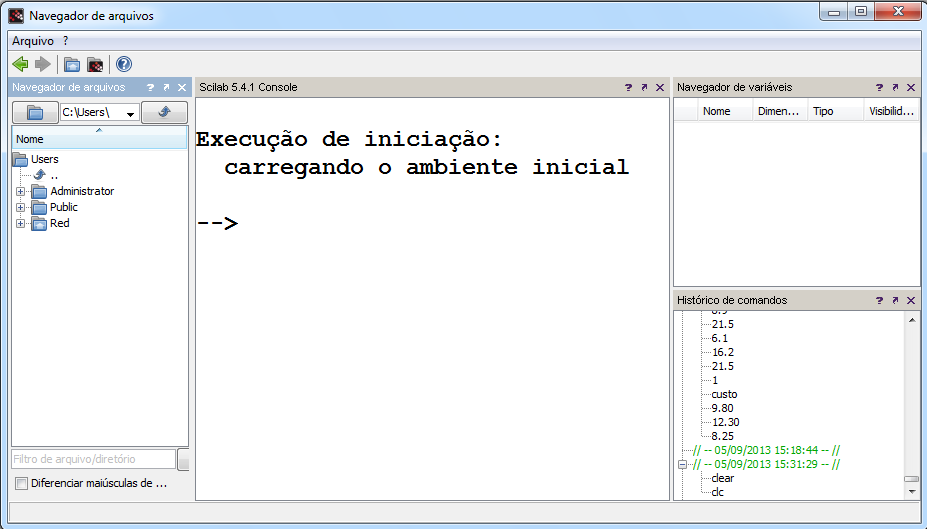
\includegraphics[width=\textwidth]{images/ambiente.png}
\end{frame}

\begin{frame}[fragile,allowframebreaks]{O console}
  \begin{itemize}
    \item Permite a inserção de comandos interativamente.
    \item O scilab apresenta o \alert{\emph{prompt}} \verb|--->| para
    sinalizar que está aguardando a digitação de um comando.
    \item O usuário digita o comando e pressiona \verb|<ENTER>|.
    \item O Scilab executa o comando e exibe a resposta.
    \item Exemplos de interação no console:
    \begin{pygmented}[lang=text]
--> 57/4
 ans  =
    14.25
--> (2+9)^5
 ans  =
    161051.
---> area = %pi * 2.5^2
 area =
    19.6350
    \end{pygmented}
    \pyginline|ans| significa \emph{answer} -- resposta.

    \framebreak
    
    \item Uma instrução pode começar em uma linha e continuar em linhas
    subsequentes colocando \verb|...| no fim das linhas incompletas.
    \begin{pygmented}[lang=text]
---> x1 = 10 + 2.36 - 89.6 * 125 + 14 - 2.986
 x1  =
    19.79

---> x2 = 10 + 2.36 - 89.6 * ...
--->      125 + 14 - 2.986
 x2  =
    19.79
    \end{pygmented}
  \end{itemize}
\end{frame}

\begin{frame}[fragile,allowframebreaks]{O histórico de comandos}
  \begin{itemize}
    \item A \alert{janela de histórico de comandos} exibe uma lista dos
    comandos que o usuário executou no console.
    \item Os comandos ficam na lista até serem deletados.
    \item Para executar novamente um comando, basta efetuar um clique
    duplo com o botão esquerdo do mouse.
    \item Para deletar um ou mais comandos da Janela de Histórico de
    Comandos, selecione o comando e efetue um clique com o botão direito
    do mouse. Um menu popup será exibido e permitirá a exclusão do
    comando.
  \end{itemize}
  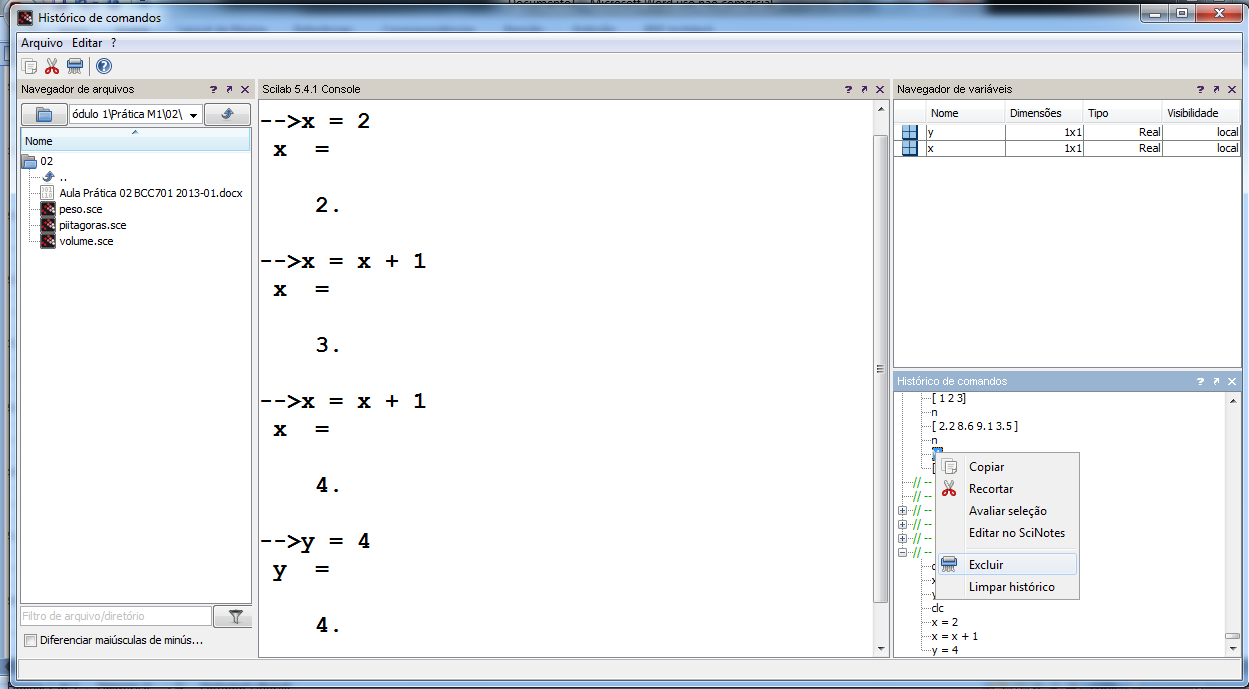
\includegraphics[width=\textwidth]{images/historico.png}
\end{frame}

\begin{frame}[fragile,allowframebreaks]{A janela de edição}
  \begin{itemize}
    \item A \alert{janela de edição} (\textbf{SciNotes}) é usada para
    criação de novos arquivos, programas Scilab, ou para modificação de
    arquivos existentes.
    \item Os seguintes passos são realizados para criação de um arquivo
    no SciNotes:
    \begin{itemize}
      \item Clique no ícone referente ao SciNotes:
      \begin{center}
        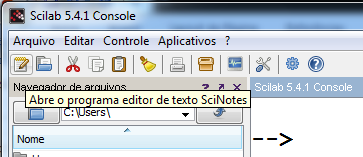
\includegraphics[scale=0.5]{images/scinotes1}
      \end{center}
      \item Digite o programa na Janela do SciNotes;
      \item Clique no ícone para salvar o arquivo; forneça um nome de
      arquivo com a extensão \texttt{sce}.
      \begin{center}
        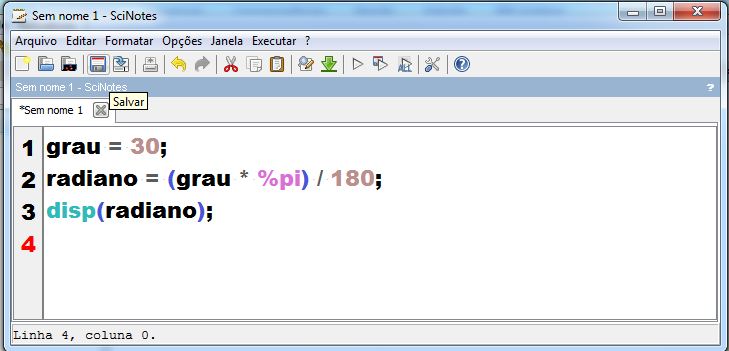
\includegraphics[scale=0.3]{images/scinotes2}
      \end{center}
      \item Escolha o diretório para salvar o arquivo:
      \begin{center}
        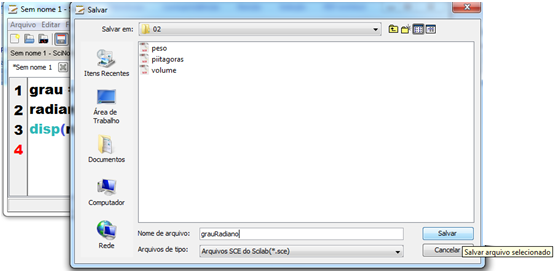
\includegraphics[scale=0.5]{images/scinotes3.png}
      \end{center}
      \item Clique no ícone para executar o programa e veja o resultado
      exibido na Janela do Console:
      \begin{center}
        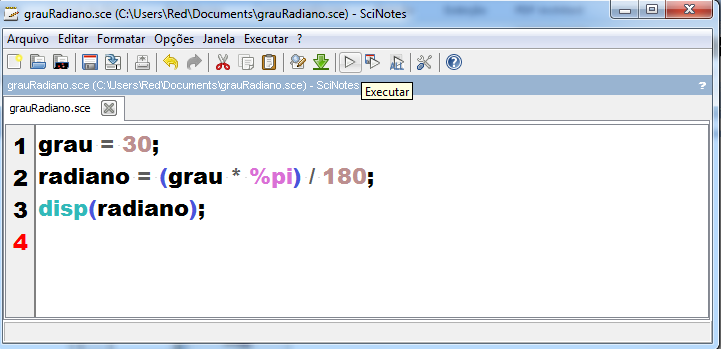
\includegraphics[scale=0.32]{images/scinotes4.png}
      \end{center}
    \end{itemize}
    \item Resultado na janela do console:
    \begin{center}
      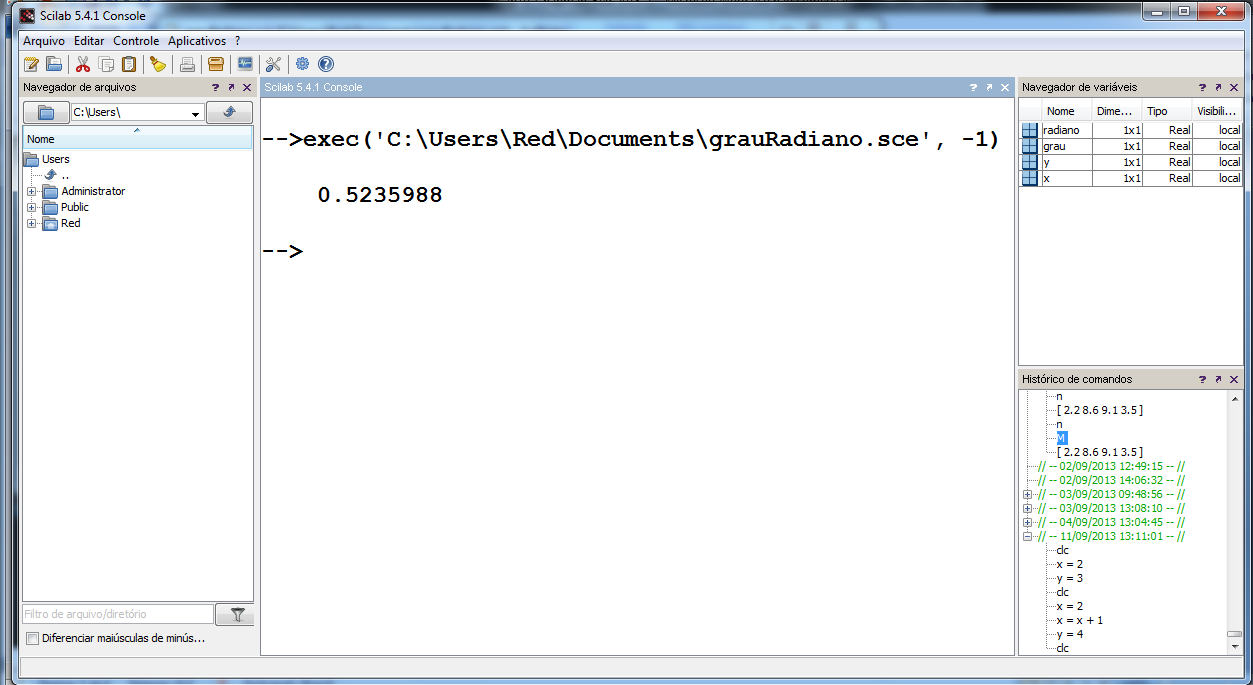
\includegraphics[width=0.9\textwidth]{images/scinotes5.png}
    \end{center}
  \end{itemize}
\end{frame}

\begin{frame}[fragile,allowframebreaks]{O ambiente de trabalho do Scilab}
  \begin{itemize}
    \item Um comando \texttt{x = 20} cria uma variável denominada
    \texttt{x}, armazena nela o valor \texttt{20}, e a salva em uma
    parte da memória do computador conhecida como \textbf{ambiente de
      trabalho}.
    \item O ambiente de trabalho é uma \alert{coleção de todas as
      variáveis}, e arrays, que podem ser utilizados em um comando
    particular ou em um programa Scilab.
    \item Todos os comandos, e arquivos, executados no console,
    \alert{compartilham} um ambiente de trabalho comum.
    \item Logo eles \alert{compartilham todas as variáveis}.
    \item A \alert{janela do navegador de variáveis} exibe todas as
    variáveis do ambiente em um dado momento.
    \item Uma \alert{lista de variáveis e arrays} armazenados no
    ambiente de trabalho corrente pode ser gerada com o comando
    \texttt{whos}.
    \item Exemplo:
    \begin{pygmented}[lang=text]
---> raio = 2; volume = (4/3) * %pi * raio^3;
---> whos
Nome                     Tipo           Tamanho        Bytes        

%T                       boolean        1 por 1        24           
%t                       boolean        1 por 1        24           

raio                     constant       1 por 1        24           

volume                   constant       1 por 1        24           
whos                     function                      15416        
    \end{pygmented}
    \begin{center}
      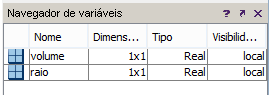
\includegraphics[]{images/whos.png}
    \end{center}
    \item Note que as variáveis raio e volume estão no mesmo ambiente de
    trabalho, podendo ser usadas por qualquer programa Scilab.
    \item O \alert{conteúdo} de qualquer variável do ambiente de
    trabalho pode ser determinado digitando-se o nome da variável no
    console.
    \begin{center}
      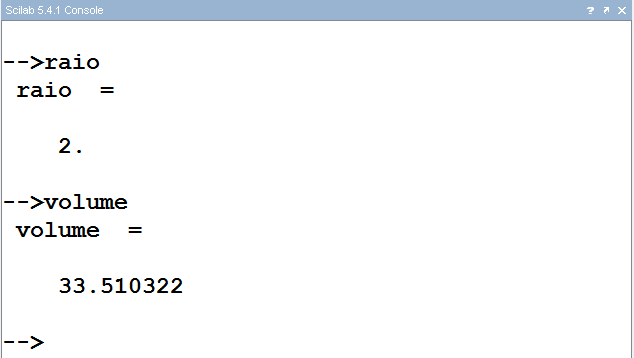
\includegraphics[width=0.6\textwidth]{images/conteudo.png}
    \end{center}
    \item Uma variável pode ser \alert{deletada}, ou apagada, do
    ambiente de trabalho através do comando \texttt{clear}:
    \begin{center}
      \texttt{clear var1, var2, ...}
    \end{center}
    onde \texttt{var1} e \texttt{var2} são nomes de variáveis a serem
    deletadas.
    \begin{center}
      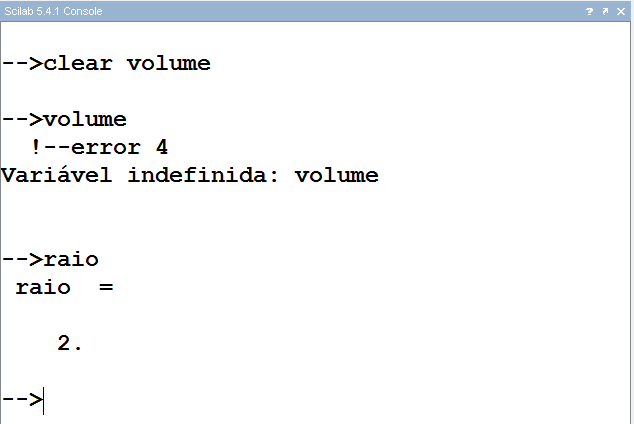
\includegraphics[scale=0.4]{images/clear.png}
    \end{center}
    \item O comando \texttt{clear}, sem mencionar as variáveis, limpa
    todas as variáveis do ambiente de trabalho.
    \begin{center}
      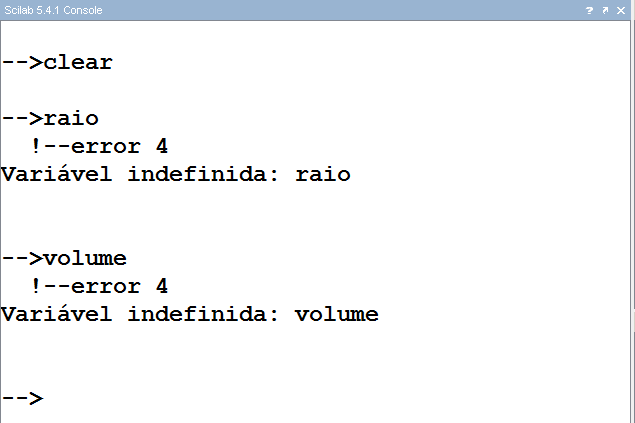
\includegraphics[scale=0.4]{images/clear2.png}
    \end{center}
  \end{itemize}
\end{frame}

\begin{frame}[fragile,allowframebreaks]{Buscando ajuda}
  \begin{itemize}
    \item A forma mais simples de buscar ajuda no Scilab é através do
    \textbf{Navegador de Ajuda}.
    \begin{center}
      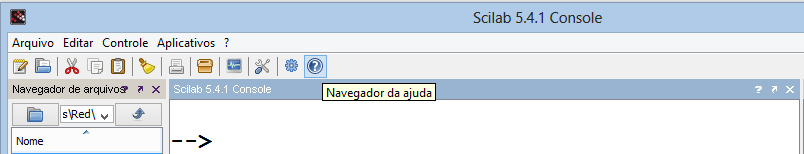
\includegraphics[width=0.9\textwidth]{images/ajuda1.png}
    \end{center}
    \item Através do Navegador de Ajuda pode-se \alert{consultar} os
    detalhes de funcionamento de um comando particular.
    \item Por exemplo, consultando-se o comando \texttt{clc}:
    \begin{center}
      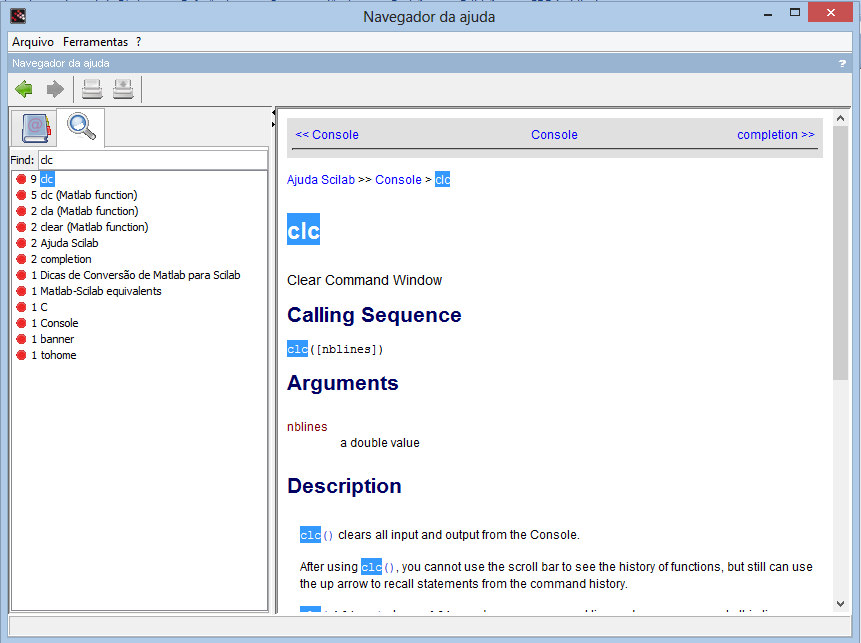
\includegraphics[scale=0.4]{images/ajuda2.png}
    \end{center}
    \item Também, pode-se digitar no Console o comando exibido abaixo,
    obtendo-se a mesma janela.
    \begin{center}
      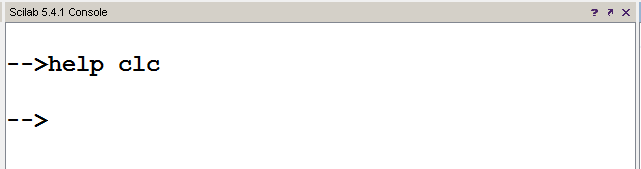
\includegraphics[scale=0.4]{images/ajuda3.png}
    \end{center}
  \end{itemize}
\end{frame}

\begin{frame}[fragile,allowframebreaks]{Alguns comandos importantes}
  \begin{description}
    \item[\texttt{clc}] limpa a janela do console do Scilab, apagando
    toda a entrada e saída da mesma.

    \item[\texttt{clear}] limpa o ambiente de trabalho do Scilab, ou
    seja, remove todas as variáveis não protegidas.

    \item[\texttt{abort}] interrompe a avaliação atual e retorna ao
    estado inicial do prompt no console, permitindo sair de situações de
    erro.

    \item[resume] retoma a execução da tarefa que estava sendo executada
    sem sair de situação de erro.
  \end{description}
\end{frame}

\begin{frame}[fragile,allowframebreaks]{Usando o Scilab Como Um Bloco de Notas}
  \begin{itemize}
    \item Em sua forma mais simples, o Scilab pode ser usado com um
    bloco de notas para \alert{efetuar cálculos}.
    \item Os cálculos são realizados digitando-se diretamenteno prompt
    as expressões matemáticas.
    \item Algumas operações matemáticas e suas respectivas
    representações simbólicas no Scilab
    \begin{center}
      \begin{tabular}{lll}\hline
        operação matemática & representação no Scilab & exemplo \\ \hline
        adição & \texttt{+} & \texttt{2 + 8}\\
        subtração & \texttt{-} & \texttt{3 - 9}\\
        multiplicação & \texttt{*} & \texttt{19 * 7.8}\\
        divisão & \texttt{/} & \texttt{8.88 / 0.0001}\\
        potenciação & \texttt{\textasciicircum} & \texttt{2 \textasciicircum (1/3)}\\
        \hline
      \end{tabular}
    \end{center}
    \item Exemplo: cálculo da área de um círculo dada pela fórmula:
    \[ A = \pi r^2 \] onde $r$ é o raio do círculo. Supondo que o
    raio seja 5cm, temos:
    \begin{center}
      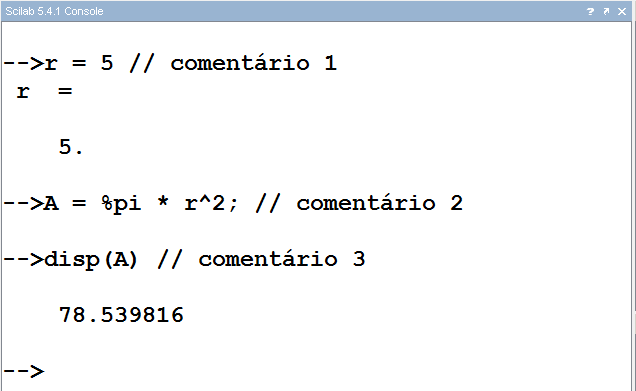
\includegraphics[scale=0.4]{images/area.png}
    \end{center}
    \item Tudo que for escrito após \texttt{//} é \alert{ignorado} pelo
    Scilab.
    \item Esta é a forma de se escrever um \textbf{comentário} em um
    código Scilab.
    \item O comentário tem a função de \alert{esclarecer} alguma coisa
    importante para o programador.
    \item Exemplo: cálculo do volume de um cilindro cuja base é um
    círculo de área igual $A$, e cuja altura é $h = 4cm$
    \begin{center}
      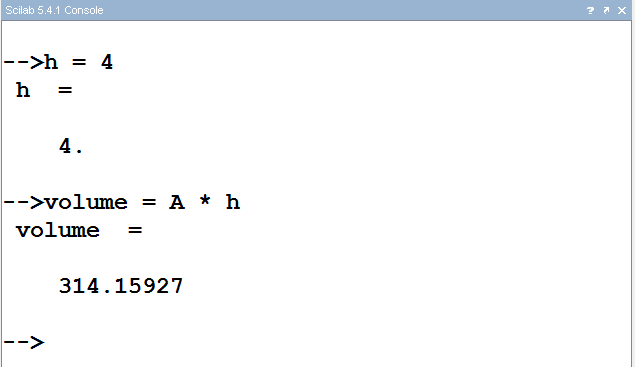
\includegraphics[scale=0.4]{images/volume.png}
    \end{center}
  \end{itemize}
\end{frame}

\begin{frame}[fragile,allowframebreaks]{Formatação para exibição de números: formato variável}
  \begin{itemize}
    \item \textbf{Formato variável} é a formatação padrão, com tamanho
    máximo de 10 posições para o número exibido, reservando uma posição
    para o ponto decimal e outra para o sinal.

    \item Por exemplo:
    \begin{pygmented}[]
--> x = 1.3456789012345
 x  =
      1.3456789
    \end{pygmented}
    o numero impresso tem 10 posições, sendo uma para o sinal:

    \framebreak

    \item Além disso, é possível definir a saída de um processamento
    numérico em função de seu tamanho, através do comando
    \alert{format}:
    \begin{center}
      \texttt{format(n)}
    \end{center}
    onde \texttt{n} é o tamanho total, incluindo o ponto decimal e o
    sinal.

    \item Por exemplo:
    \begin{pygmented}[]
--> format(15)
--> x
 x  =
      1.345678901235
    \end{pygmented}
    redefine o formato para o tamanho 15 (com doze decimais).
  \end{itemize}
\end{frame}

\begin{frame}[fragile,allowframebreaks]{Formatação para exibição de números: formato científico}
  \begin{itemize}
    \item \textbf{Formato científico}: O comando
    \begin{center}
      \texttt{format('e')}
    \end{center}
    redefine o formato para \texttt{'e'}, com a saída exibida no formato
    científico.

    \item O valor exibido é truncado na oitava casa decimal, onde
    \texttt{D+00} significa \emph{10 elevado a 0}, que é igual a 1.

    \item Por exemplo:
    \begin{pygmented}[]
--> format('e')
--> x
 x  =
     1.34567890D+00
    \end{pygmented}

    \item Agora, vamos redefinir a saída padrão com 10 posições:
    \begin{pygmented}[]
--> format('v', 10)
--> x
 x  =
     1.3456789
    \end{pygmented}
  \end{itemize}
\end{frame}

\begin{frame}{Exercícios}
  \begin{exercise}
    A distância percorrida por uma bola em queda livre no ar é dada pela
    equação:

    \[ x = x_0 + v_0 t + \frac{1}{2} a t^2 \]

    Utilize o Scilab para calcular a posição da bola no tempo $t = 5 s$,
    se $x_0 = 10 m$, $v_0 = 15 m/s$ e $a = -9,81 m/s^2$ .
  \end{exercise}

  \begin{exercise}
    Suponha que $x = 3$ e $y = 4$. Utilize o Scilab para avaliar as
    seguintes expressões matemáticaS:
    \begin{enumerate}
      \item \[ \frac{x^2 y^3}{(x - y)^2} \]
      \item \[ \frac{1}{x^2 - y} - e^{-4x} + \sqrt[3]{\frac{35}{y}} \sqrt{xy} \]
    \end{enumerate}
  \end{exercise}
\end{frame}

\begin{frame}
  \begin{center}
    Fim
  \end{center}
\end{frame}

\end{document}

%%% Local Variables:
%%% mode: latex
%%% TeX-master: t
%%% End:
